\documentclass[12pt]{article}
\usepackage[a4paper, total={6in, 9in}]{geometry}
\usepackage[utf8]{inputenc}
\usepackage{amsmath}
\usepackage{graphicx}
\usepackage{listings}
\usepackage{subfig}
\usepackage{floatrow}
\usepackage{hyperref}
\usepackage{sectsty}

\sectionfont{\fontsize{12}{15}\selectfont}
\begin{document}
\title{A3- Unsupervised Learning Report}
\author{Dheekshitha PS}
\textbf{A3- Unsupervised Learning} \\


In this assignment, we are exploring and analysing different unsupervised learning algorithms for clustering and dimensionality reduction. 


\section{Data 1-Customer Churn Prediction}

The first data used is the same binary classification data from assignment 1 called Customer churn prediction data. This data was highly imbalanced as 83.5:16.5 ratio of classes. There are 10k rows with 23 features with 5 categorical variables which are one-hot encoded for the experiments. Using SMOTE, the the minority class samples are synthetically generated. The target variable is now in 2:1 ratio. This dataset is intresting in terms of assignemnt3 because the data is a binary class one and I would like to see how clustering might give the results. Is it going to be 2 clusters or more than that is what I am excited to see.

\section{Data 2-White wine quality}

The second data I used is the White Wine quality data. This data has been chosen to see how clustering works on multi label data.This data has class labels (quality) ranging from 3 - 9. The data has 4898 rows with 11 features. The classes are not uniformly spread instead huge variation is present. Dominant class is Class 6 with ~2K records and the least is class 9 with 5 records. This makes me wonder if clustering can form 7 clusters or less than that.


\section{Clustering approach}

In this set of experiments, K-means clustering and Expected Maximization,a Gaussian Mixture Model have been done on both the datasets. 
\subsection{K means}
K-means clustering works by randomly intializing a centroid and then assigning each datapoint into one of clusters based on distance(eg:Euclidean, Manhattan). In the next step, it evaluates the clusters and then picks a different centroid for this group of data points. This is iteratively until the algorithm converges.	
\subsection{Expected Maximization}
Expected Maximization is a type of soft clustering which means the data points are not assigned to cluster but rather the probability of belonging to each of the cluster is given. EM is a Gaussian Mixture Model where 2 step approach of Expectation of log-likelihood followed by maximizing that likelihood is done.

The following approach is taken in builing and evaluating the K-means clusters in the parts 1 and 3. 
\begin{itemize}

\item Standardise and normalised the data as K-means clustering depends on distance between the points
\item Clusters in the range of 2 to number of features were built using Euclidean distance
\item Chose the best cluster number based on WCSS-Within Cluster Sum of Squared Errors, Silhouette scores and Silhoutte vizualization
\item Clusters were vizualised by T-sne or pair plots of features that are important. The important features were obtained by random forest feature importance

\end{itemize}

In case of Expected Maximization(called EM going further)-
\begin{itemize}

\item Standarised and normalised data was used
\item Number of components and  covariance type(spherical, diagonal, tied or full) parameters were tuned
\item BIC-Bayesian information criterion is used to find the optimal number of clusters
\end{itemize}
Covariance type in EM helps in constraining the covariance of the difference. BIC is used as the performance metric as it penalises the number of parameters to avoid overfitting. In sklearn implementation of EM, the model with least BIC is the best one.

\*Note-Silhouette score curves and elbow curves are not plotted for all the experiments because of space constraint.


\section{Part 1}

In this part, 2 types of clustering models were built as per the approach defined above. As shown in the figure , none of the features in the original datasets are truely different for different class labels. For data1, the features 3,4,5 looked important but they are also overlapping for 2 labels in the data. 
As per figure 1, there is a conflict in number of clusters suggested by WCSS and Silhouette scores. In figure2, Silhouette visualizations, all the different number of cluster graphs have some clusters with silhouette scores negative. However, in 16 clusters graph, all the clusters width is similar. Hence 16 clusters were built for data1. Though the original data was binary class, the clusters suggested by all the 3 approaches was suprisingly 16.\\

Similarly for data2, the 4 cluster graph has all the clusters with Silhouette score more than average score and the width is almost same. Hence 4 clusters were built. In the T-SNE graph, Figgure 4B, the clusters are very well segregated in 12 and 2 dimesions. However, the intra cluster distance is more in case of 2 dimesions rather than 12 for data2.\\
In case of EM, the number of components were 5 with diag covariance type for data 1 and 	9 components with full covariance type for data2. For data2, the number of components were more than the actual number of classes. The BIC value kept decreasing as the number of components increased in case of data2 . The EM cluster vizualization for both the data clearly shows the ellipsoid clusters formed by EM in constrant to circular by Kmeans. Kmeans clusters as vizualised in T-sne graph show that the clusters are well seperated out in 2 dimesions rather than in actual 32 dimensions.

\begin{figure}[htbp]
    \centering
    \subfigure[a]{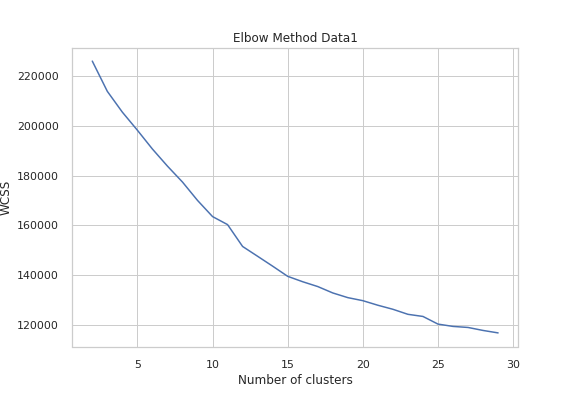
\includegraphics[width=0.2\textwidth]{kmeans1_WCSS.png}} 
    \subfigure[b]{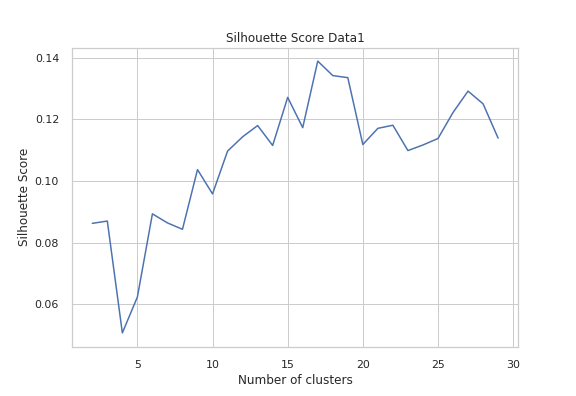
\includegraphics[width=0.2\textwidth]{kmeans1_SScore.png}} 
    \subfigure[c]{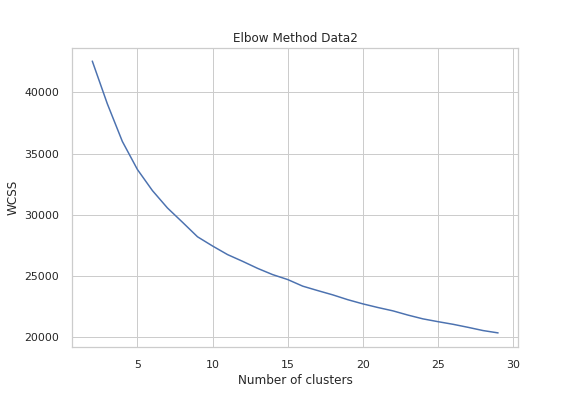
\includegraphics[width=0.2\textwidth]{kmeans2_WCSS.png}}
    \subfigure[d]{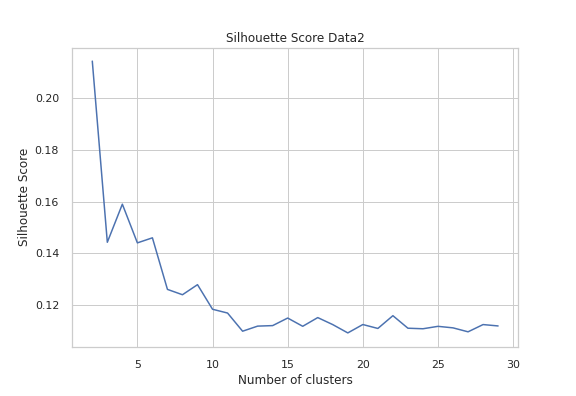
\includegraphics[width=0.2\textwidth]{kmeans2_SScore.png}}
    \caption{[K Means Elbow curve using WCSS & Silhouette Score] LEFT:Data1, RIGHT:Data2 }
    \label{fig:foobar}
\end{figure}


\begin{figure}[htbp]
    \centering
    \subfigure[a]{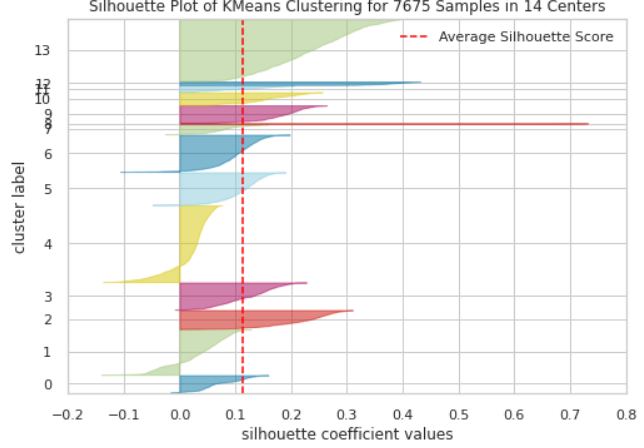
\includegraphics[width=0.2\textwidth]{sv_data1_1.png}} 
    \subfigure[b]{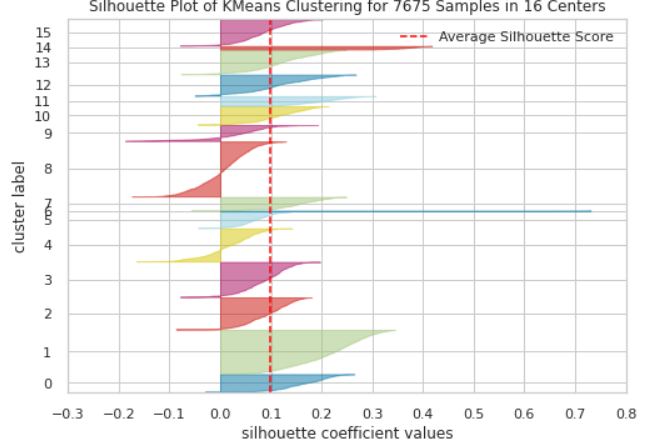
\includegraphics[width=0.2\textwidth]{sv_data1_2.png}} 
    \subfigure[c]{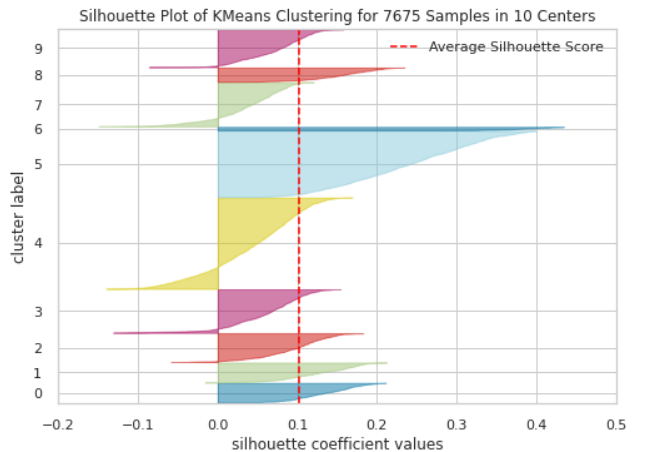
\includegraphics[width=0.2\textwidth]{sv_data1_3.png}}
    \subfigure[d]{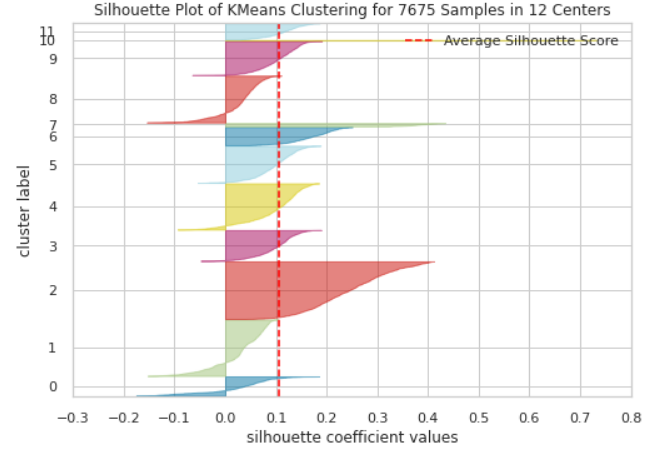
\includegraphics[width=0.2\textwidth]{sv_data1_4.png}}
    \caption{Silhouette Vizualization for different cluster numbers-Data1 }
    \label{fig:foobar}
\end{figure}

\begin{figure}[htbp]
    \centering
    \subfigure[a]{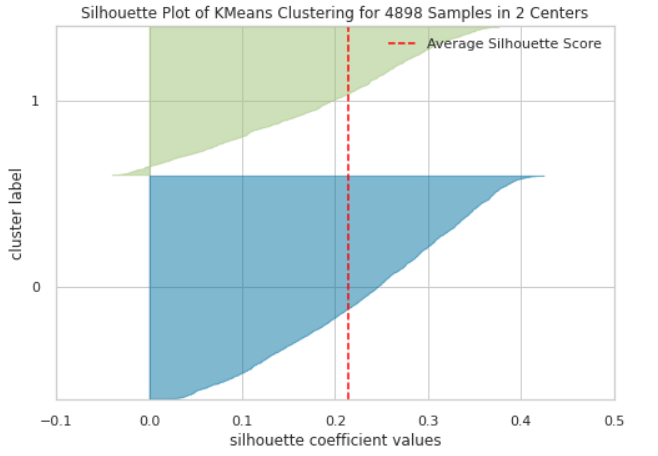
\includegraphics[width=0.2\textwidth]{sv_data2_1.png}} 
    \subfigure[b]{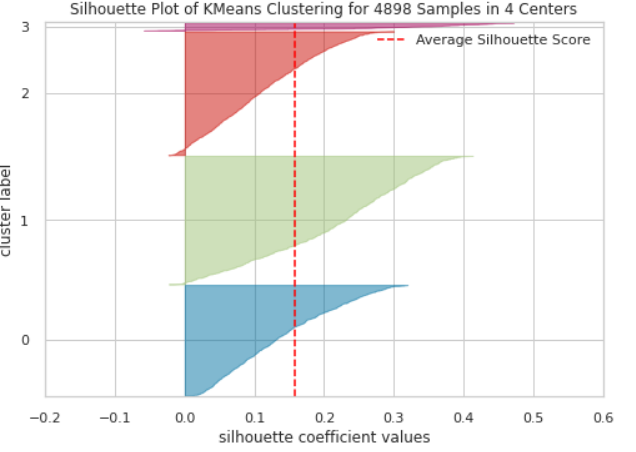
\includegraphics[width=0.2\textwidth]{sv_data2_2.png}} 
    \subfigure[c]{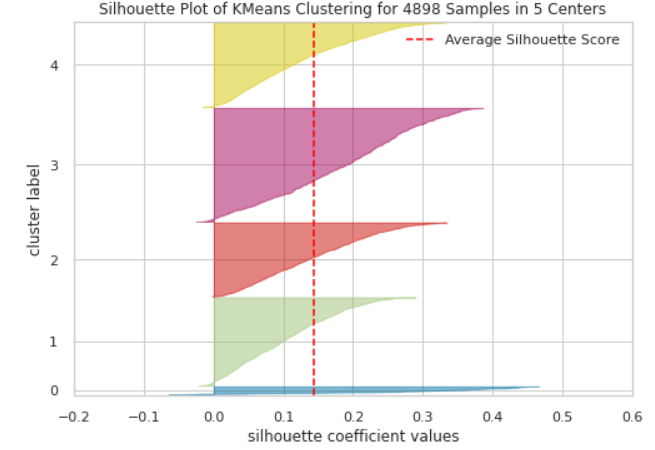
\includegraphics[width=0.2\textwidth]{sv_data2_3.png}}
    \subfigure[d]{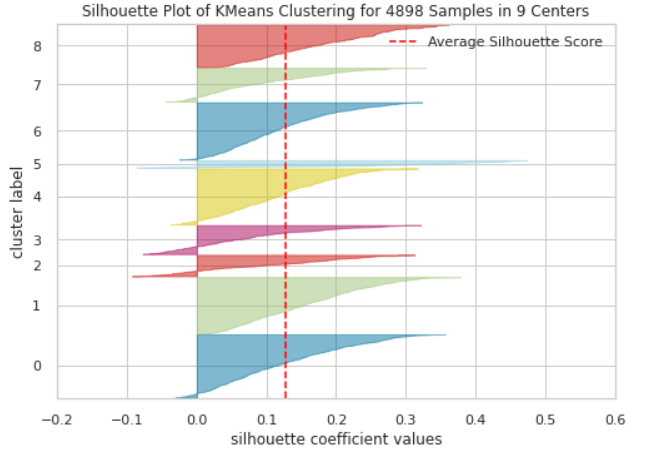
\includegraphics[width=0.2\textwidth]{sv_data2_4.png}}
    \caption{Silhouette Vizualization for different cluster numbers-Data2 }
    \label{fig:foobar}
\end{figure}


\begin{figure}[htbp]
    \centering
    \subfigure[a]{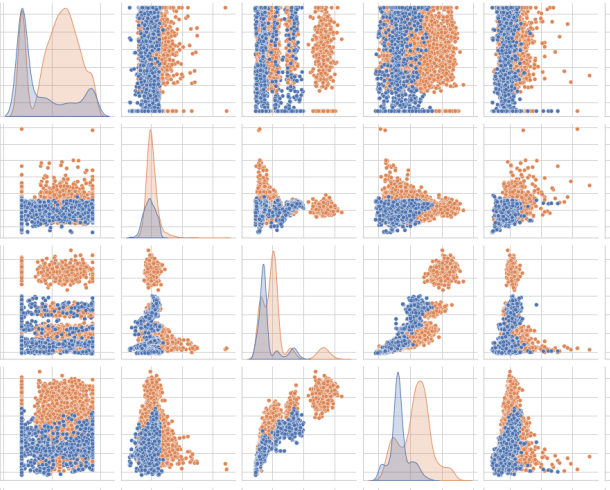
\includegraphics[width=0.2\textwidth]{crooped_Data1.png}} 
    \subfigure[b]{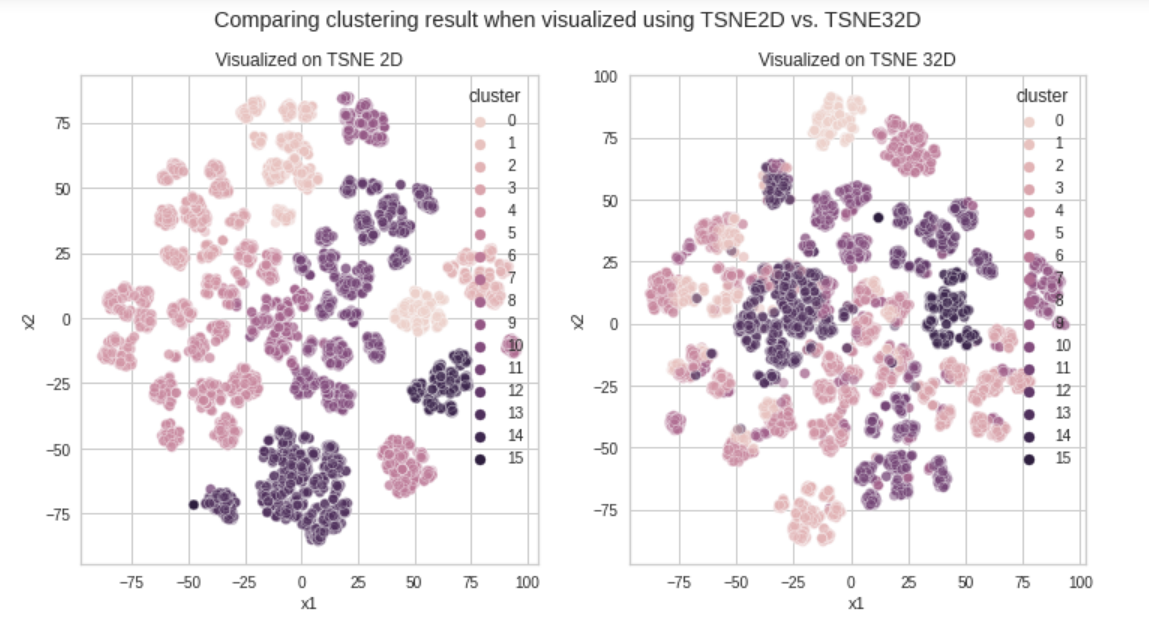
\includegraphics[width=0.2\textwidth]{part1_Kmeanstsne.png}} 
    \subfigure[c]{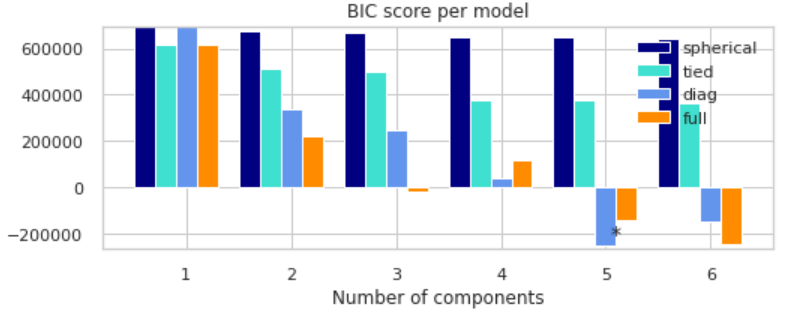
\includegraphics[width=0.2\textwidth]{part1_BIC.png}}
    \subfigure[d]{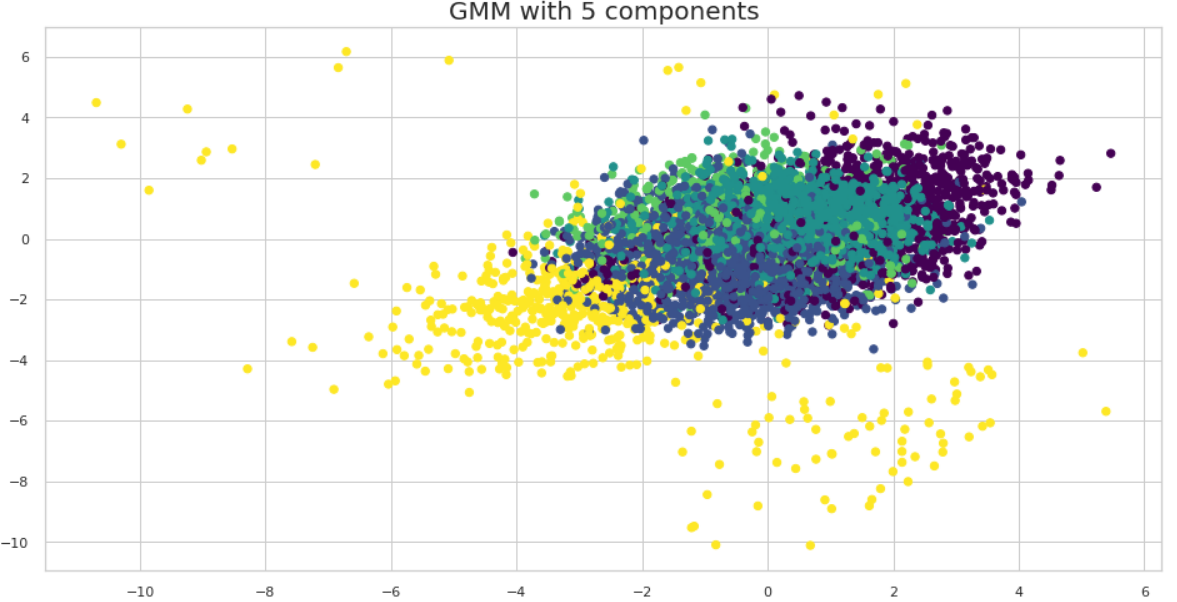
\includegraphics[width=0.2\textwidth]{emviz_data1.png}}
    \caption{Data1 -a)Pairplot on original data b)T-sne Vizualization c) BIC curve EM d)EM Vizualization }
    \label{fig:foobar}
\end{figure}






\begin{figure}[htbp]
    \centering
    \subfigure[a]{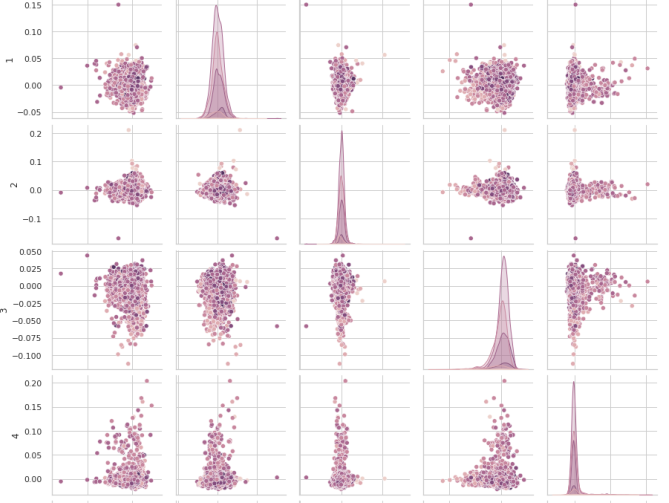
\includegraphics[width=0.2\textwidth]{croppedFeatures_Data2.png}} 
    \subfigure[b]{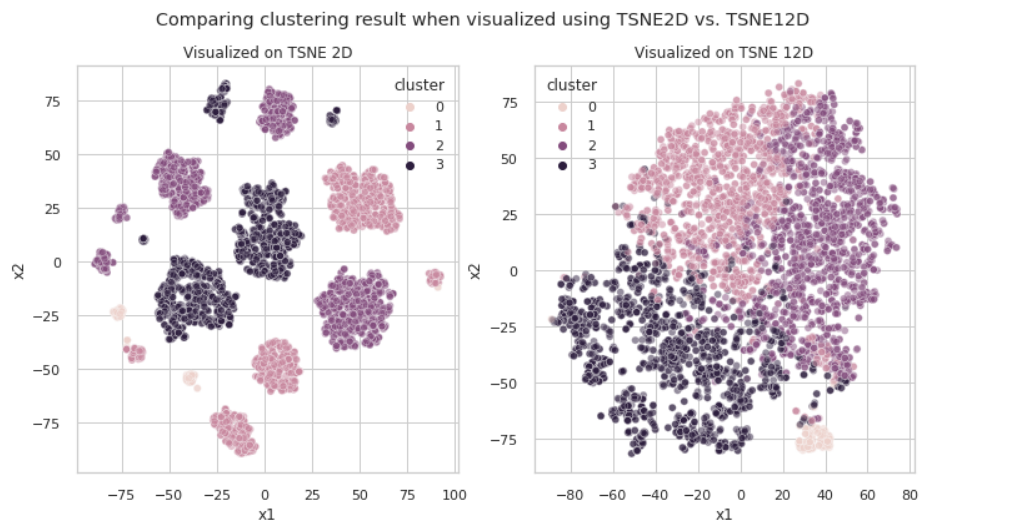
\includegraphics[width=0.2\textwidth]{tsne_data2_km.png}} 
    \subfigure[c]{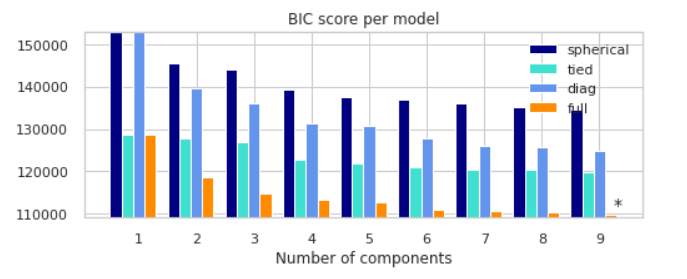
\includegraphics[width=0.2\textwidth]{BIC_Data2.png}}
    \subfigure[d]{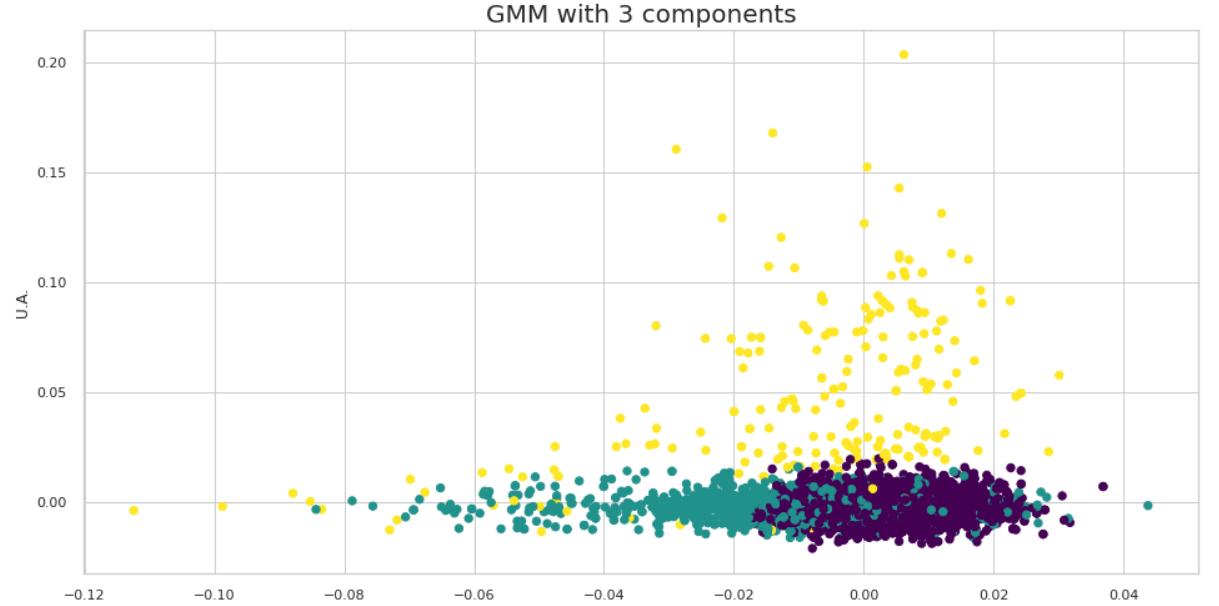
\includegraphics[width=0.2\textwidth]{emviz_data2.png}}
       \caption{Data2 -a)Pairplot on original data b)T-sne Vizualization c) BIC curve EM d)EM Vizualization }
    \label{fig:foobar}
\end{figure}

\subsubsection*{Part 1 Conclusion}
Number of clusters, number of components and covariance type are tuned to get better results.From the experiments above, the model clustered a binary class data in 16 clusters and a multi(7) class data into 3 clusters. This clearly tells us that the unsupervised clustering techniques   cannot exactly be replace supervised models as unsupervised techniques are tending to find different patterns in the data and not necessarily the target variable. Also we can notice that if there is no underlying pattern in the original data as in the case of data1, the model cannot also find the pattern and cluster well.
\section{Dimensionality reduction approach}
In the parts 2,4 dimensionality reduction was done as per the following approach-
\begin{itemize}

\item Principal Compenent Analysis(PCA) was done by varying number of principal components. Number of optimal principal components were chosen based on the cumulative explained variance
\item In Independent Component Analysis(ICA), mean Kurtosis was used a metric to chose the right number of components

\item Gaussian Random Projection(RP) was performed by using the Mean Reconstruction Correlation and Reconstruction error. Mean reconstruction correlation is taken as the mean correlation in the newly produced projection should be same as the mean correlation in the original space
\item The 4th algorithm chosen for dimensionality reduction is kernel PCA. Kernel PCA can perform complex nonlinear projections for dimensionality reduction. This method retains the clusters of instances after projection. Different kernels like rbf and sigmoid were tried



\end{itemize}


\section{Part 2 and 3}
In this part, 4 dimensionality reduction techniques were applied and clustering was done on top the reduced data as per the approaches defiend above. 
\subsection{PCA}
\subsubsection*{Dimensionality Reduction}
For data1, the number of components requried to get 95 \% of cummulative explained variance was 23 and 8 in case of data2. The cummulative explained variance by the first two components for data1 is less than 20 \% whereas it is 43 \%. This clearly tells us that there are no specific compoents for data1 that are strongly explaning the data. The scatter plot for the first two PCs also shows that the first two PCs are not enough to clearly separate the data. However, data2 with 43 \% of explanined varaince also couldn't differentiate actual class lables. This implies that when the class labels are more, more variance is required to differniate them.
\subsubsection*{Clustering analysis}
In the clustering analysis using PCA data, the number of clusters for K-means given by elbow and silhoutte curves was same as before i.e 16. The clusters for EM were 9. From figure 7a and 7b, it is evident that EM did well in making elliposidal clusters on PCA data rather than K-means. However, this is exactly opposite in case of data 2 where K-means nicely clustered the data, EM's ellipsoids look a little cluttered.


\begin{figure}[htbp]
    \centering
    \subfigure[a]{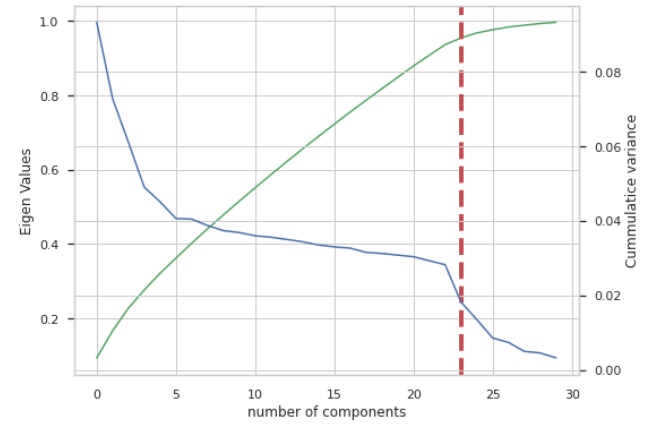
\includegraphics[width=0.2\textwidth]{pca_cumm_new.png}} 
    \subfigure[b]{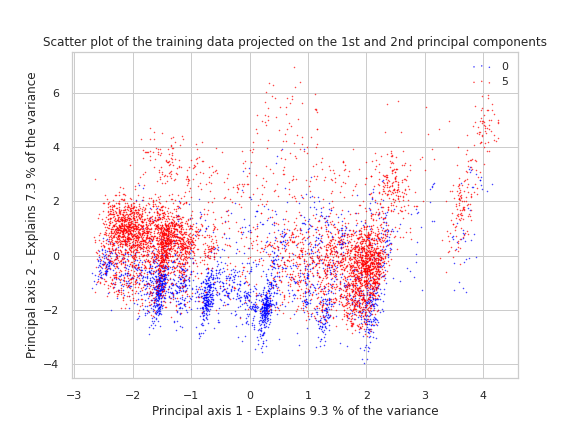
\includegraphics[width=0.2\textwidth]{pca_data1_scatter.png}} 
    \subfigure[c]{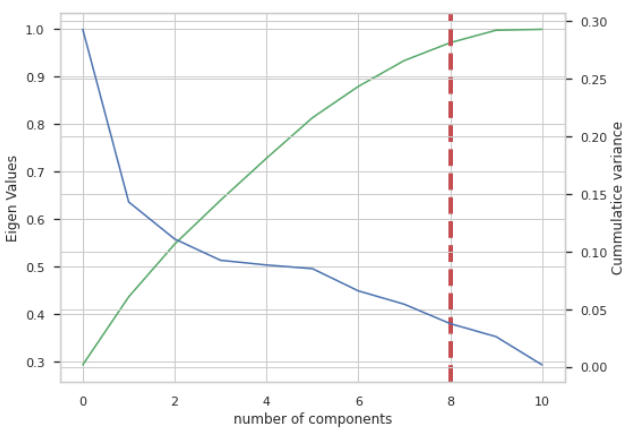
\includegraphics[width=0.2\textwidth]{pca_data2_cumm_NEW.png}}
    \subfigure[d]{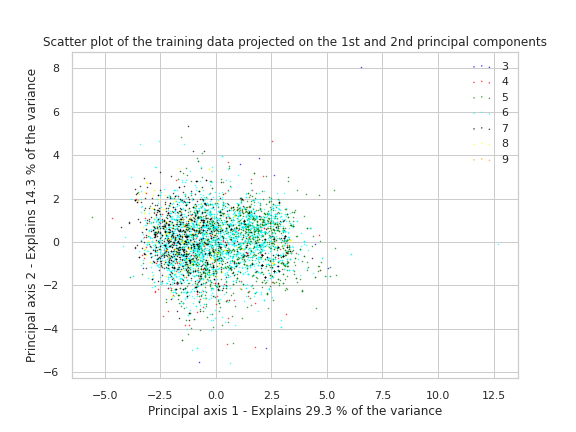
\includegraphics[width=0.2\textwidth]{pca_data2_Com12.png}}
    \caption{[Cummulative variance curves and scatter plot for PCA]LEFT:Data1 RIGHT
    :Data2}
    \label{fig:foobar}
\end{figure}

\begin{figure}[htbp]
    \centering
    \subfigure[a]{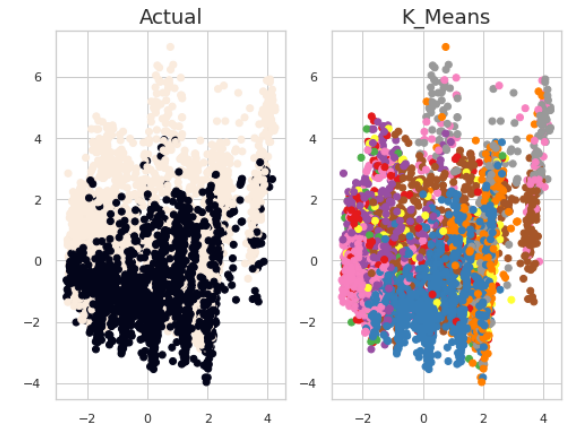
\includegraphics[width=0.2\textwidth]{pca_data1_kmeans.png}} 
    \subfigure[b]{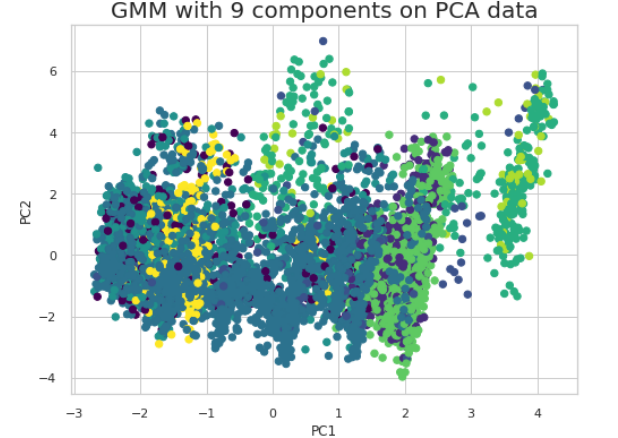
\includegraphics[width=0.2\textwidth]{data1_pca_emVIZ.png}} 
    \subfigure[c]{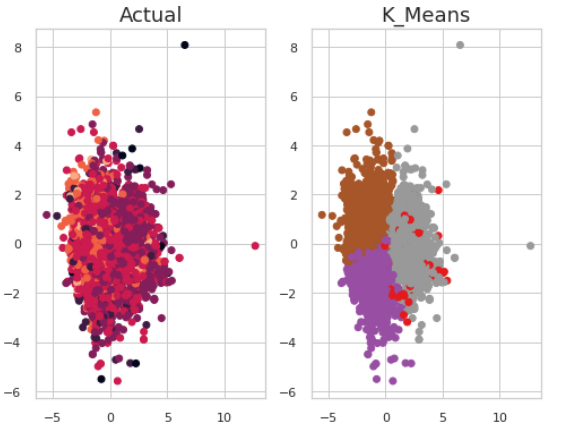
\includegraphics[width=0.2\textwidth]{data2_pca_kmeans.png}}
    \subfigure[d]{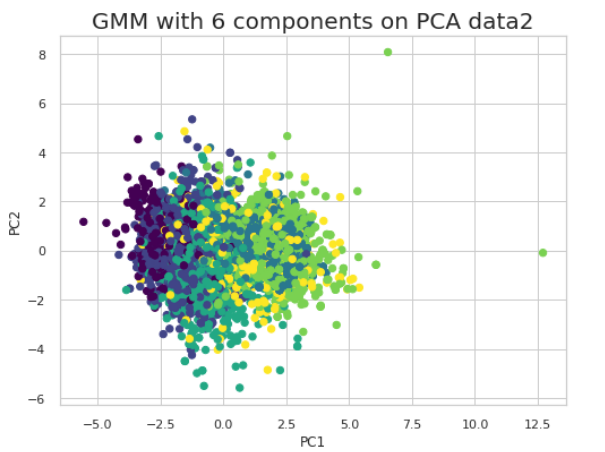
\includegraphics[width=0.2\textwidth]{data2_emVIZ.png}}
    \caption{[Kmeans and EM vizualization-PCA]LEFT:Data1 RIGHT
    :Data2}
    \label{fig:foobar}
\end{figure}

\subsection{ICA}
ICA in contrast to PCA tries to reduce the data into independent orthogonal components in the new space. This is done by increasing the seperation between each of the components.High kurtosis represents highly independent components hence this is used as a metric to choose optimal components. Based on the Fig 8a, 23 components were initially chosen for data1. On closer analysis, it is found that not all the components have good mean kurtosis. There are components with negligible(when compared with other components) mean kurtosis that were removed but keeping the order of components intact. Only 6 out of 23 components and 5 out of 10 components were chosen for data 1 and data 2 respectively.\

As seen in Figure 9a and 9b, ICA was able to find the independent components very well. All the clusters it formed are clearly independent. However,same is not true in case of data. Data2 still looks	messy. 
\begin{figure}
    \centering
    \subfigure[a]{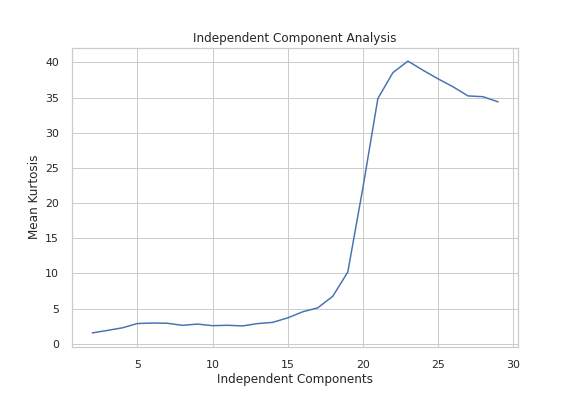
\includegraphics[width=0.2\textwidth]{ica_data1_kurt.png}} 
    \subfigure[b]{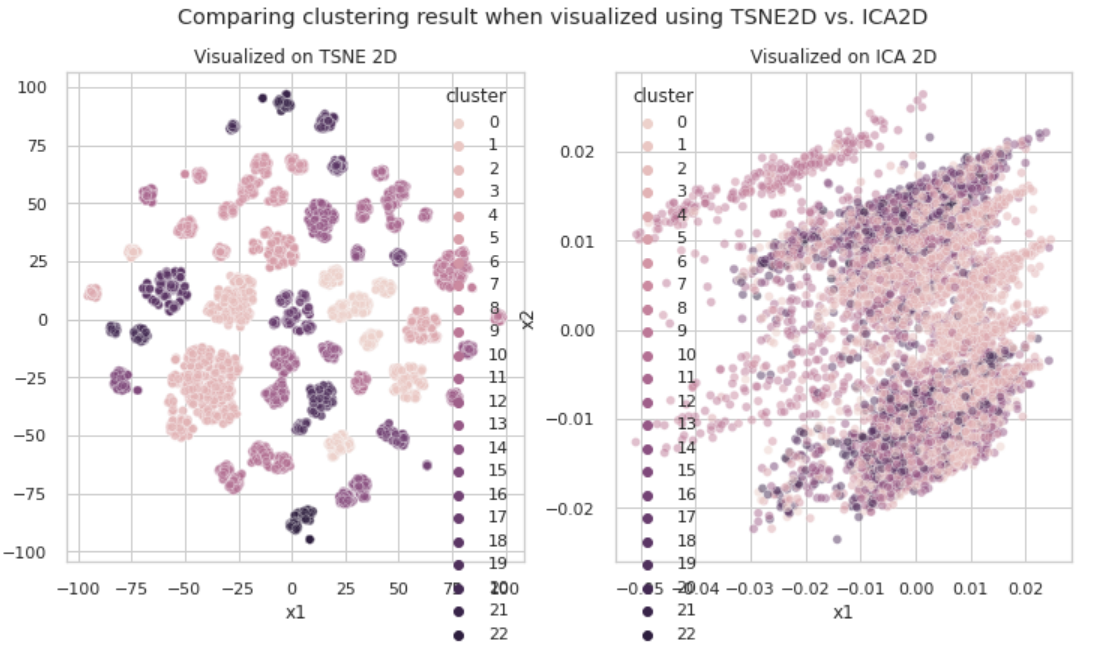
\includegraphics[width=0.2\textwidth]{icatsne_data1.png}} 
    \subfigure[c]{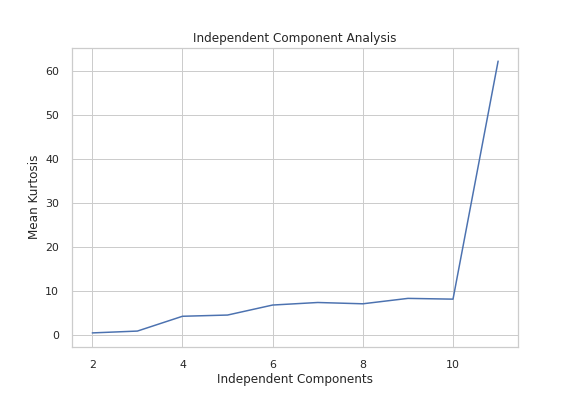
\includegraphics[width=0.2\textwidth]{pca_data2_ICA.png}}
    \subfigure[d]{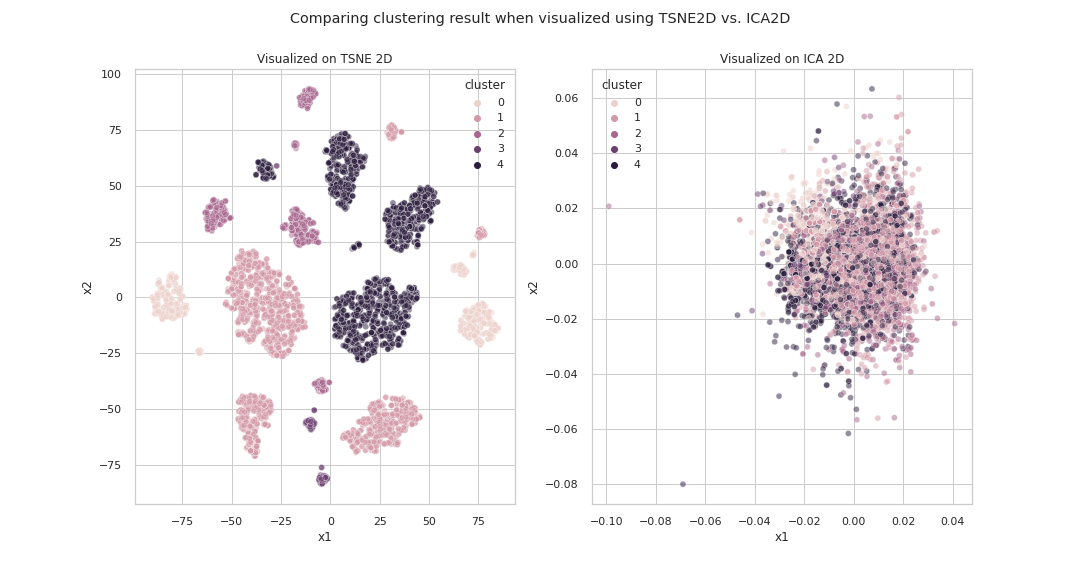
\includegraphics[width=0.2\textwidth]{data2_ICA_tsne.png}}
    \caption{[ICA curves- Mean Kurtosis and T-sne vizualization] LEFT:Data1 RIGHT:Data2 }
    \label{fig:foobar}
\end{figure}






\begin{figure}
    \centering
    \subfigure[a]{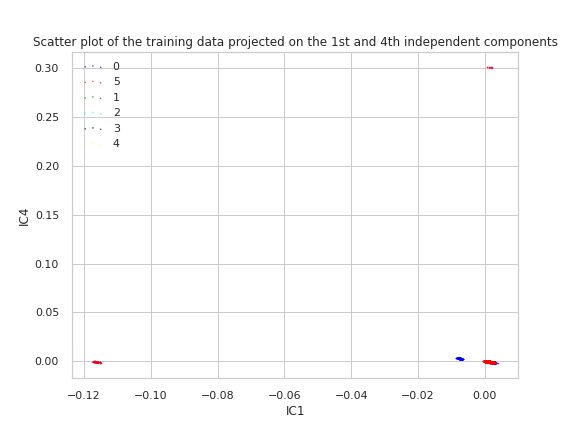
\includegraphics[width=0.2\textwidth]{Ica_data1_scatter_km.png}} 
    \subfigure[b]{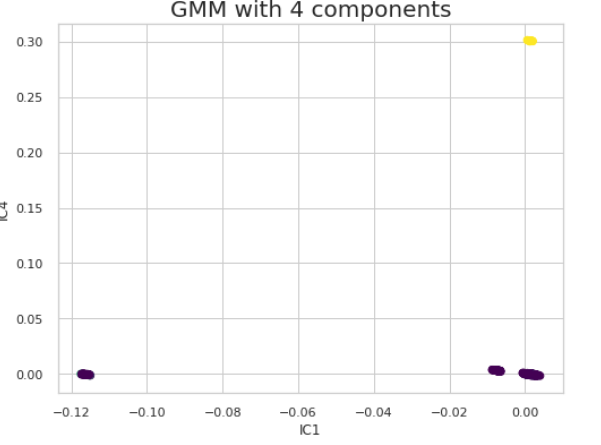
\includegraphics[width=0.2\textwidth]{ica_data1_em.png}} 
    \subfigure[c]{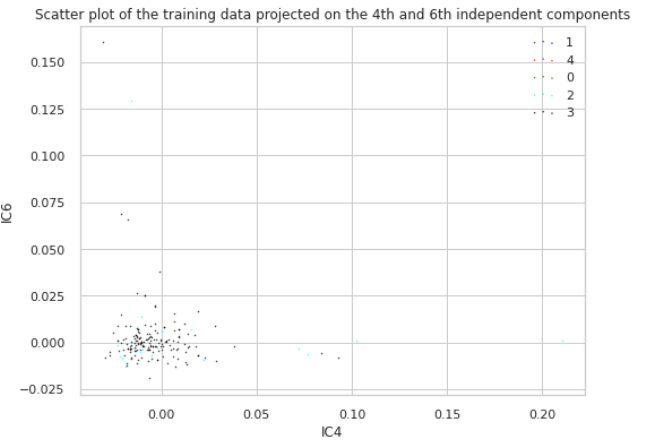
\includegraphics[width=0.2\textwidth]{Ica_data2_scatter_km.png}}
    \subfigure[d]{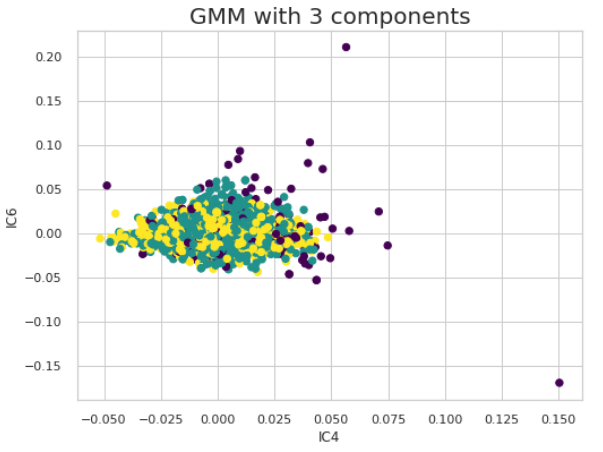
\includegraphics[width=0.2\textwidth]{ica_data2_em.png}}
    \caption{[ICA curves- Scatter plot of important components] LEFT:Data1 RIGHT:Data2 }
    \label{fig:foobar}
\end{figure}


\subsection{Random Projection}
This is the 3rd dimensionality reduction technqiue that is used. This algorithm works by randomly projecting data into new space but in a different direction. But the new dimension must be less than the actual dimension of the data. As this is a random approach, this algorithm is run with different random states.\\

The metric used to find the optimal number of components is reconstruction error(called RMSE going forward) and mean reconstruction correlation. RMSE is obtained by reconstructing the data from the randomly projected data and calculating  the Root mean sqaured error. 
Figure 10b and 10c show that the reconstruction error calculated is fluctutaing a lot as the number of components increase. But they are forming normal distribution like patterns at periodic intervals. This could be because I am using gaussian random projection.\\

In the clusters built on randomly projeceted data, the scattered plot of first two components look very neat and seperated. The clusters formed are much better than PCA and ICA. This applies to both kmeans and EM on both the datasets. This comes as a surprise to me as models like PCA or ICA could not give such good results when compared to random projections.

\begin{figure}[htbp]
    \centering
    \subfigure[a]{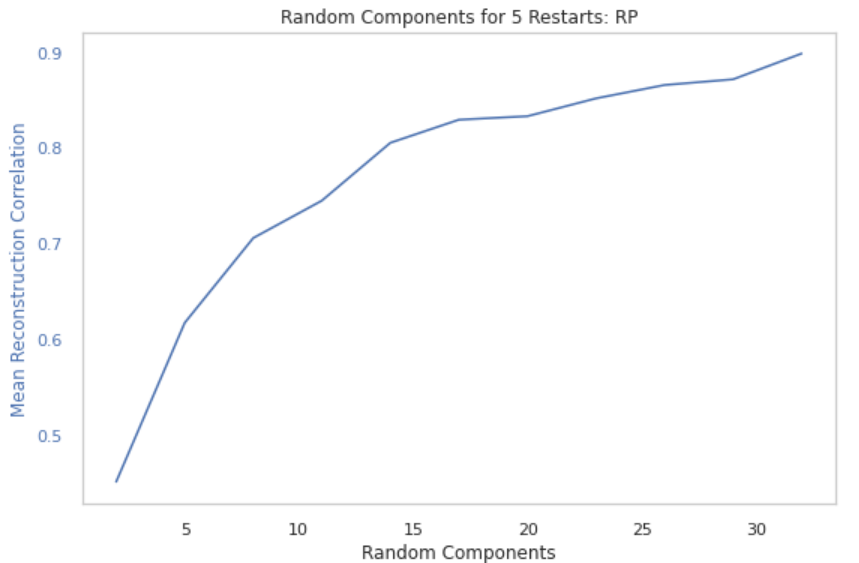
\includegraphics[width=0.2\textwidth]{rca_Data1.png}} 
    \subfigure[b]{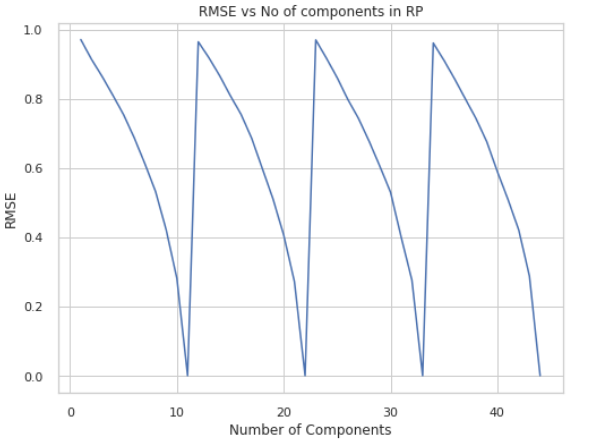
\includegraphics[width=0.2\textwidth]{rmse_rp_curve.png}} 
    \subfigure[c]{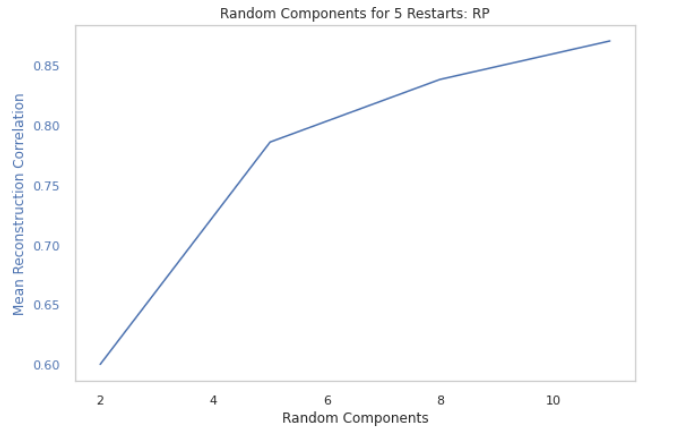
\includegraphics[width=0.2\textwidth]{rca_Data2.png}}
    \subfigure[d]{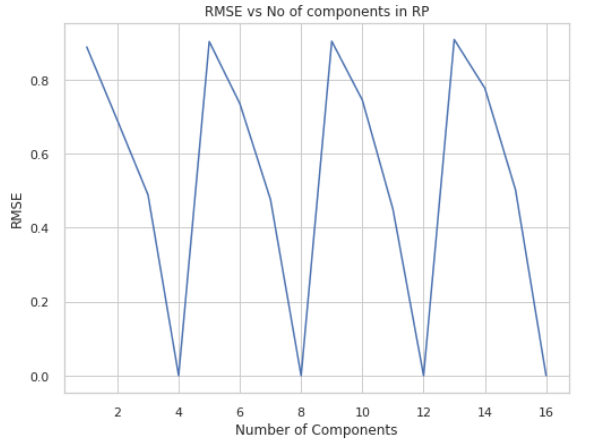
\includegraphics[width=0.2\textwidth]{rmse_data2RP.png}}
    \caption{[Random Projection curves- RMSE and Mean Correlation] LEFT:Data1 RIGHT:Data2 }
    \label{fig:foobar}
\end{figure}







\begin{figure}[htbp]
    \centering
    \subfigure[a]{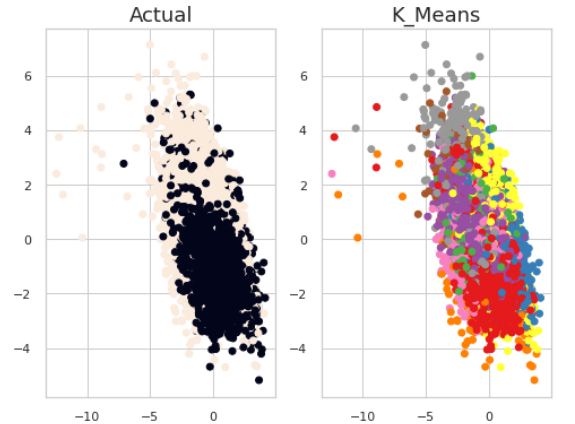
\includegraphics[width=0.2\textwidth]{data1_rp_kmeans.png}} 
    \subfigure[b]{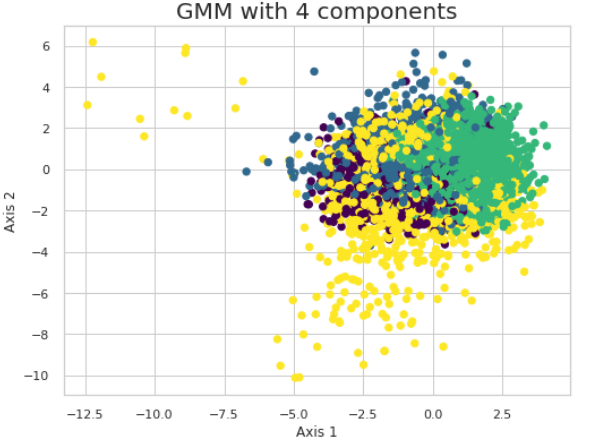
\includegraphics[width=0.2\textwidth]{data1_rca_em.png}} 
    \subfigure[c]{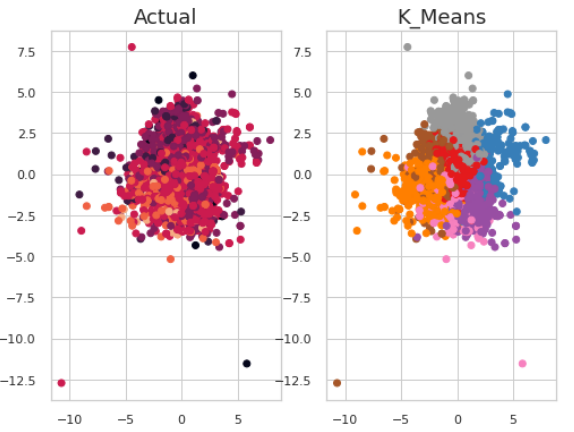
\includegraphics[width=0.2\textwidth]{data2_rca_kmeans.png}}
    \subfigure[d]{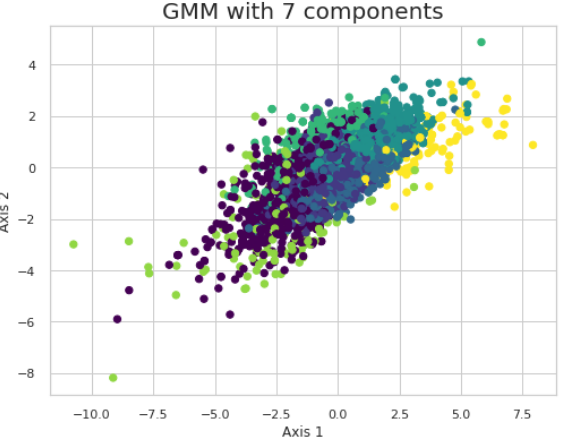
\includegraphics[width=0.2\textwidth]{data2_rca_em.png}}
    \caption{[Random Projection curves- Scatter plot of important components] LEFT:Data1 RIGHT:Data2 }
    \label{fig:foobar}
\end{figure}

\subsection{Kernel PCA}
The 4th dimensionality reduction technqiue that is chosen is KernelPCA.This alogirthm is chosen as this forms complex non-linear dimensions when compared to linear in PCA. Different kernels in kernel PCA can be used as per the data. Similar to SVM kernels, in kernel PCA as well the data is projected into different dimension as per the kernel chosen.






\begin{figure}[htbp]
    \centering
    \subfigure[a]{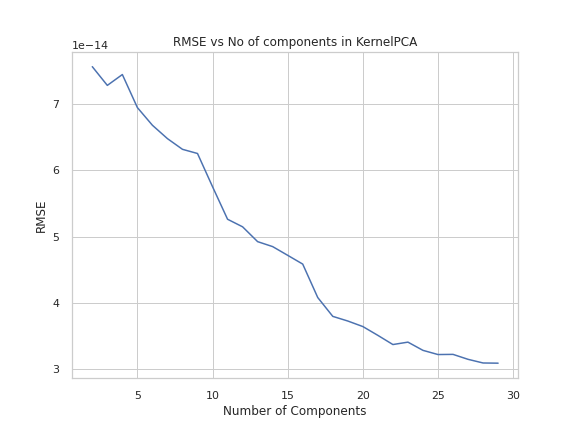
\includegraphics[width=0.2\textwidth]{rmseKernel.png}} 
    \subfigure[b]{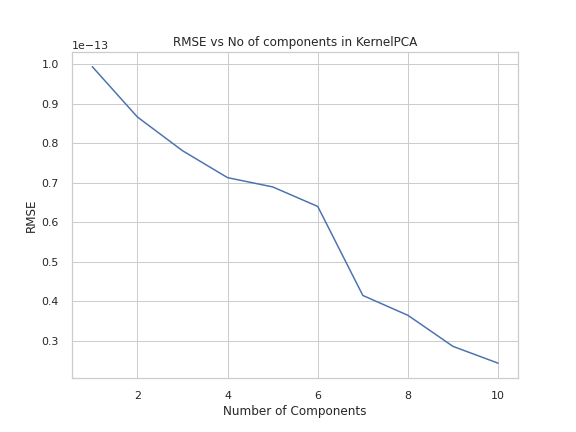
\includegraphics[width=0.2\textwidth]{data2_rmseKernel.png}} 
    \subfigure[c]{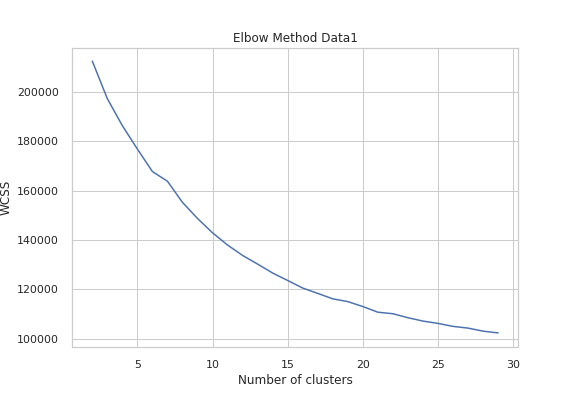
\includegraphics[width=0.2\textwidth]{kpca_data1_wcss.png}}
    \subfigure[d]{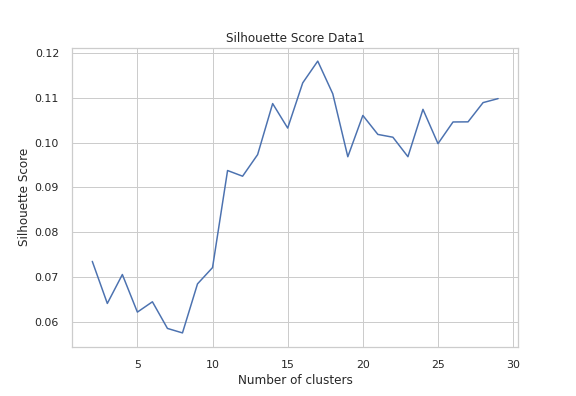
\includegraphics[width=0.2\textwidth]{KPCA_data1_Sscore.png}}
    \caption{[Kernel PCA curves- Scatter plot of important components] LEFT:Data1 RIGHT:Data2 }
    \label{fig:foobar}
\end{figure}


\begin{figure}[htbp]
    \centering
    \subfigure[a]{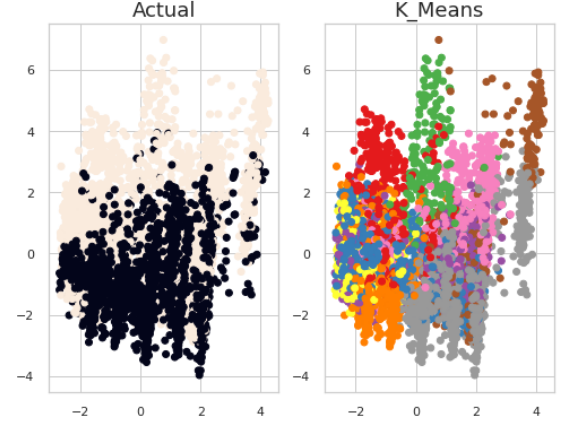
\includegraphics[width=0.2\textwidth]{kpca_Data1_Kmeans.png}} 
    \subfigure[b]{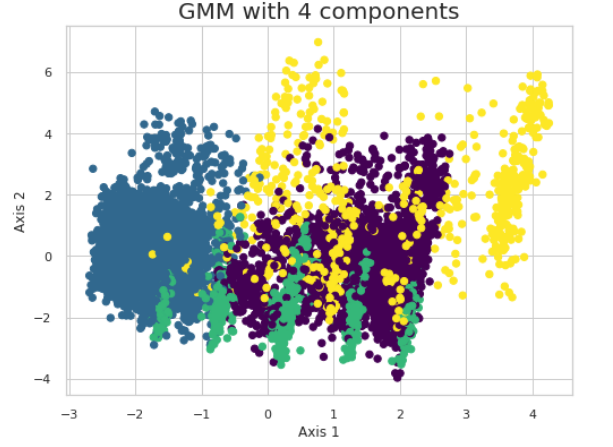
\includegraphics[width=0.2\textwidth]{kpca_Data1_em.png}} 
    \subfigure[c]{\includegraphics[width=0.2\textwidth]{kpca_Data2_Kmeans.png}}
    \subfigure[d]{\includegraphics[width=0.2\textwidth]{kpca_Data2_em.png}}
    \caption{[Kernel PCA curves- Scatter plot of important components] LEFT:Data1 RIGHT:Data2 }
    \label{fig:foobar}
\end{figure}

\subsubsection*{Part2 and 3 Conclusion}
In these 2 parts, dimensionality reduction techniques are applied on both the datasets and hyperparameters were chosen by using performance metrics like reconstruction error,BIC, cummulative explained variance etc. Clustering is done on top of the reduced data. Significant imprvoment in the clusters fromed is noticed especially in RP and KernelPCA. However, a common test like running  a supervised alogirthm on top of this data can actually help us understand the   power of all these algorithms.\\
One important observation to note is that though the data2 has only 11 features, non of the DR techniques were able to significantly reduce the dimensions to 2 or 3. But with data 1 having 32 features, the reduction was higher.


\section{Part 4}
In this section, neural network was run on the data 1 i.e. Customer churn prediction which is dimensionally reduced in part 2. Gridsearch was done on hidden layers and learning rate to find the optimal parameters and further hyper parameters were tuned. Precision is used as the performance metric in assignment 1 hence going forward with the same.\\

 I expect data reduced using KPCA outperfrom the other three datasets as the reconstruction error for KPCA was very minisicule. The clusters formed when KPCA was applied first were vizually much better than other algorithms.


Dimensionally reduced data was further normalised before training the model. The test and validation data were transformed on the already built models from part 2. Though PCA has reduced the dimension of the data from 32 to 23, the number of hidden layers that were required to get performance were more than what was required for original data. \\

Random projection performed worst of all the algorithms and also when compared to original data. This could be because, the train data was randomly projected and the same model was used on validation data which might not have generalised well. Surprisingly, KPCA did not outperform and stood 4th out of 5. The performance was less on both train and validation data. Not sure why this is happening. PCA stood second interms of performance and first in terms of speed. Though PCA had highest number of features(componenets) when compared to all the 3, it managed to outperform. However, original data took highest runtime than any others which is as expected because of higher dimensionality.






\begin{figure}[htbp]
    \centering
    \subfigure[a]{\includegraphics[width=0.2\textwidth]{LC_PCA.png}} 
    \subfigure[b]{\includegraphics[width=0.2\textwidth]{LC_ICA.png}} 
    \subfigure[c]{\includegraphics[width=0.2\textwidth]{LC_RP.png}}
    \subfigure[d]{\includegraphics[width=0.2\textwidth]{lc_kpca.png}}
    \caption{Learning Curves for data1-PCA,ICA,RP,KPCA}
    \label{fig:foobar}
\end{figure}


 \begin{center}
  \begin{table}
 \begin{tabular}{|c| c| c| c|c|c|} 
  \hline
Data & PCA & ICA & RP & KPCA & OriginalData\\ [0.5ex] 
 \hline
 Data1-Train & 26 &28 &144 & 28& 145\\ 
 
 Data1-Prediction& 0.22&0.2 &21 & 0.09& 0.12 \\ [1ex] 
 \hline
\end{tabular}
\caption{\label{tab:table-name}Precision for different experiments-Part4}
\end{table}

\end{center}


\begin{center}
 \begin{table}
 \begin{tabular}{||c| c| c| c|c|c||} 
 \hline
Data & PCA & ICA & RP & KPCA & OriginalData\\ [0.5ex] 
 \hline\hline
 Train&94 & 89 & 76 &87 &98 \\ 
 \hline\hline
 Validation&92&92 & 83& 88& 95\\ [1ex] 
 \hline\hline

\end{tabular}
\caption{\label{tab:table-name}Precision for different experiments-Part4}
\end{table}

\end{center}

\subsubsection*{Part 4 Conclusion}
In neural network model on reduced data, PCA outperformed all the others but less than original data. This could be because though PCA or any other dimensionality reduction technique reduce the runtime when there are 100s of features, they might not always capture the entire pattern in original data. We can use these technqiues at the cost of little amount of accuracy/precision for the computation cost.


\section{Part 5}
In this part, clustered data from part1 is used along with the predicted labels to build the neural network. As we are adding the information of predicted cluster label to the data, I expect the models to outperform or match the performance of original data. The number of features after one hot encodin the cluster labels is 32 in case of K-means and 10 in case of EM. So the runtime should ideally be less for EM when compared to the other two.\\

From the below table, none of the clustered data outperformed the original data.This could be because the clustering we did is segregating the data into multiple classes /clusters.But the neural network is trying to do a binary classification. This could be one of the reasons why adding cluster labels to the data did not help.

\begin{figure}[htbp]
    \centering
    \subfigure[a]{\includegraphics[width=0.4\textwidth]{LC_Kmeans.png}} 
    \subfigure[b]{\includegraphics[width=0.4\textwidth]{LC_EM.png}} 
     \label{fig:foobar}
\end{figure}




 \begin{center}
 \begin{table}
 \begin{tabular}{||c|c|c|c||} 
  \hline
Data & K-means & Exptected Max.& OriginalData\\ [0.5ex] 
 \hline
 Data1-Train &36 & 28& 145\\ 
 
 Data1-Prediction&0.23& 0.19& 0.12 \\ [1ex] 
 \hline
\end{tabular}
\caption{\label{tab:table-name}Model Run time for different experiments-Part5}
\end{table}

\end{center}

\begin{center}
\begin{table}
 \begin{tabular}{|| c|c|c|c||} 
 \hline
Data & K-means & Exptected Max.& OriginalData\\ [0.5ex] 
 \hline\hline
 Train& 91 &87 &98 \\ 
 \hline\hline
 Validation&90& 88& 95\\ [1ex] 
 \hline\hline

\end{tabular}
\caption{\label{tab:table-name}Precision score for different experiments-Part5}
\end{table}
\end{center}

\section{Conclusion}

Different types of clustering like distance based K means, probability based Expected Maximization are run on 2 datasets.Optimal number of clusters suggested by these algorithms were very different. Various dimensionality reduction techniques like Linear PCA, gaussian based models like random projections etc were also applied on the datasets. The performance of these are analysed in bothe supervised and unsupervised tasks.


\end{document}